%!TEX root = ../template.tex
%%%%%%%%%%%%%%%%%%%%%%%%%%%%%%%%%%%%%%%%%%%%%%%%%%%%%%%%%%%%%%%%%%%%
%% chapter2.tex
%% NOVA thesis document file
%%
%% Chapter with the template manual
%%%%%%%%%%%%%%%%%%%%%%%%%%%%%%%%%%%%%%%%%%%%%%%%%%%%%%%%%%%%%%%%%%%%

\typeout{NT FILE chapter2.tex}

\chapter{State-of-the-Art}

    The realm of automated event detection and content analysis has witnessed substantial progress over the years, aiming to enhance the overall experience for viewers, sports analysts, and enthusiasts of physical sports, video games, or sports in general \cite{BroadcatedGames_analysis_LOL}\cite{RTS_soccer_analytics}. The progression has resulted in advanced software capable of identifying and categorizing multiple events within a match or gaming session. This software can provide valuable insights into the sport and create tools to better understand the performance of players or teams \cite{ComputerVisionInSports}.

    In this chapter, we will present an overview of the current state-of-the-art in event detection and classification for video games. We will delineate the various events that can occur within various gaming sessions and the challenges that arise from each. Various approaches have been developed over the years and we will review them, and compare them against the most recent works that pertain to machine learning. We will also include some of the advancements in computer vision techniques that can be of use to the to be developed solution.  

\section{Gaming and sports video analysis} 

    Many systems were created to detect events in video games. Some were implemented as fully automatic solutions and some others as semi-automatic. Still, any of them aimed to extract the most valuable information possible at each moment and translate it into a concise textual description.

    To extract all of that high-level information it is needed to collect low-level information and process them in a way that all together can translate to a particular high-level event. This low-level information can be denominated as \gls{LLF}. These \gls{LLF} allow to extract direct information from visual or audio elements, such as the progression of color in a certain element or the variation of noise in a certain frequency.

    Identifying high-level information in gaming and sports videos follows some common steps. Just as described in \cite{AutomaticEventDetectionTennis} first, it is needed to identify low-level audiovisual and textual features present in the streaming feed. Second, a sequence of those features is grouped to identify the movement of the video game character, the round of the game played, or other audiovisual components. The results from those groups are denominated \gls{MLR}, a representation of a higher level but that cannot be used to infer the events of the video. To infer those events it is needed some prior knowledge of the sport played in the feed. When the models from \gls{MLR} are processed with that knowledge the result is high-level information, denominated of \gls{HLS} where the semantic concepts are used to identify the events, for example when the colors of the screen turn grey and the character has stopped moving in a game of League of Legends it means that the character that the gamer is manipulating has died and it will be revived, as is depicted in \cite{BroadcatedGames_analysis_LOL}. The process is depicted in Figure \ref{fig:LLF_HLS_realtion} for a better understanding of the steps and the different levels of information present in a sports video.

    \begin{figure}[htbp]
        \centering
        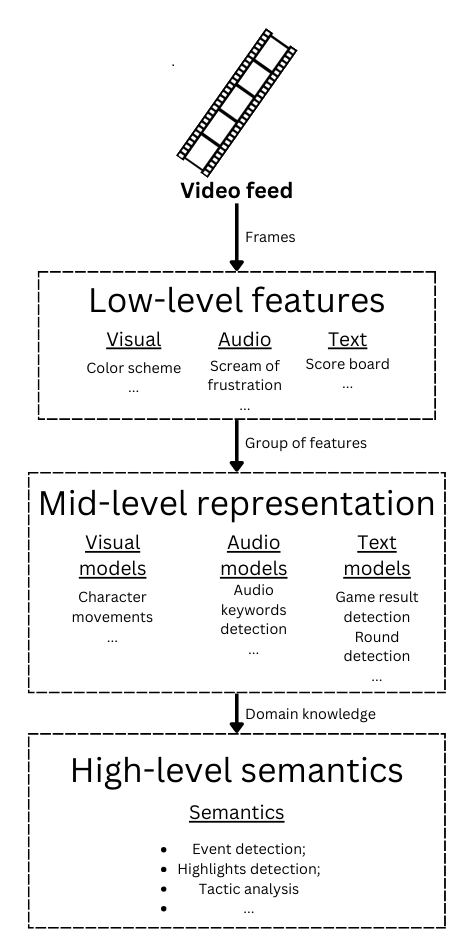
\includegraphics[width=0.7\linewidth]{Chapters/Figures/Relationship_Events.png}
        \caption{Relation between low-level features and high-level semantics (adapted from \cite{AutomaticEventDetectionTennis}}
        \label{fig:LLF_HLS_realtion}
    \end{figure}

    The following section presents a synopsis of the features present in video game feeds, as well as the strategies used to retrieve them. First, it introduces approaches made to sports videos that can be applied to video game feeds in the solution to be developed. Then it clarifies approaches already developed for video game feed and its system of event detection and highlights detection.

\subsection{Visual Patterns Analysis in Sports videos}

    Extracting visual \gls{LLF} involves obtaining information from pixel intensity values, edges, color histograms, and other elements. These features are identifiable for their ease of definition and extraction but possess limited semantic significance \cite{interaction_between_modules_in_learning_systems_for_vision_applications}. Nonetheless, relying solely on \gls{LLF} is insufficient for the development of intricate projects, such as automatic event detection due to the semantic gap.

    Therefore, to create a visual model to analyze a video game feed it is needed to rely upon \gls{MLR}. Visual \gls{MLR} are semantic concepts, which are derived from specific combinations of \gls{LLF}. In sports videos those specific combinations are related to standard camera shooting style transmission practices and domain-specific objects and their locations \cite{SOCCER_VIDEO_EVENT_DETECTION}, and in video games feeds are related to camera settings. Because the camera settings vary among individuals, the visual patterns are not identical but rather exhibit similarities.

\subsubsection*{Video event detection}

    Video event detection, highlight extraction, and summarization have been extensively researched over the years, especially regarding football. The Bagadus system \cite{RTS_soccer_analytics} effectively integrated data from multiple cameras installed in a stadium and data from sensors on football players. It provided a real-time interaction subsystem for experts to annotate soccer events. This system allows users to track specific players, view events in panorama videos, and create video summaries. Due to the high cost of expert annotations, it was developed another similar system but instead, it uses crowdsourcing to integrate annotations from crowd workers \cite{Crowd-based_Semantic_Event_Detection}. A Bayesian network-based method proposed in \cite{EventDetectionAndSummarizationInSoccerVideosUsingBayesianNetworkAndCopula} captured dependencies among extracted features based on the automatically learned joint distribution of variables for football video event detection.

    In addition to conventional highlight events like goals and penalty kicks, in \cite{SoccerVideoSummarizationCinematographyMotionAnalysis} is proposed to include scenes of intense competition and emotional moments in football video summaries. They measured the interest level of a video clip based on cinematographic and motion features. In this system, the feature analysis consisted of identifying the movement of the ball and the impact that movement had on the flow of the game. For annotating baseball videos, this article \cite{WebcastText_Baseball_Videos} aligned high-level webcast text with video content to avoid unstable performance caused by purely content-based methods. In this system, the feature analysis consisted of identifying visual features like camera movement, player movement, and ball movements, and combined with webcast text and text detected in the video resulted in tagging the pitching types. This article \cite{PlayerTrackingInBroadcastBasketballVideo} introduced a robust player tracking system and adopted player trajectories to detect highlight events and conduct tactic analysis. This system consisted of using background subtraction, edge detection, and object tracking algorithms to detect the movements of the players. After the features were obtained, it was filtered using particle filter algorithms to obtain a player tracking system. Finally, the motion analysis module analyzes it to infer statistical analysis of player movement, and events like shots made and to reconstruct the game in a 3D world simulation. Another system based on Basketball was proposed as a framework for basketball videos involving scoreboard detection, text/video alignment, and replay detection, formulated as a discrete optimization problem and solved using resource allocation approaches \cite{BasketballNovelFramework}. In comparison to the other approach, this technology used \gls{SVM} for classification tasks, such as shot boundary detection and object detection, and \gls{RF} and \gls{NN} for action and event detection.  

\subsection{Audio Patterns Analysis in Sports videos}

    The audio component of a sports video such as the voice of the commentator, music, and various kinds of environmental sounds is a very important type of media and very correlated to the video component. Various previous works on audio analysis have been developed to complement the visual component, such as \cite{AutomaticDetectionGoalSegmentsBasketball}\cite{AutomaticextractionHighlightsBaseball}\cite{AudioKeywordsSoccerVideo}.

    The most basic concept used in audio pattern analysis is the audio keyword. This concept refers to any sound that is used in a game environment to describe the actions of players, referees, commentators, and audience \cite{AudioKeywordsSoccerVideo}. As depicted in Figure \ref{fig:LLF_HLS_realtion}, audio keywords can represent aural \gls{MLR}, which combined with some domain knowledge can construct the \gls{HLS}. These representations can be generated from different audio \gls{LLF} and supported by algorithms. In \cite{AudioKeywordsSportsAnalysis} is proposed an audio keyword generation system with an adaptive \gls{HMM} to correct a previous system that compromised of a hierarchical \gls{SVM} classifier where a frame-based classification followed segments of frames of 20 ms. In this previous system, for diverse sports games, the task involved gathering substantial audio samples and manually labeling them to train keyword recognizers, thereby enhancing performance across a range of sports activities.

    As shown in \ref{fig:HMM-based_keywordGenerator}, the proposed system consists of the following steps to create \gls{HMM} probabilities. The \gls{LLF}, such as the energy and the power of a signal, and pitch features including the fundamental frequency and harmonic frequencies of a signal, are extracted and tokens are added to create an observation vector. Next, the training of the \gls{HMM} models is performed using dynamic programming. With those \gls{HMM} models obtained the next step is to select testing data to compare with the incoming audio testing. The testing audio sequence is labeled as a series of predefined audio keywords according to the maximum posterior probability.

    \begin{figure}[htbp]
        \centering
        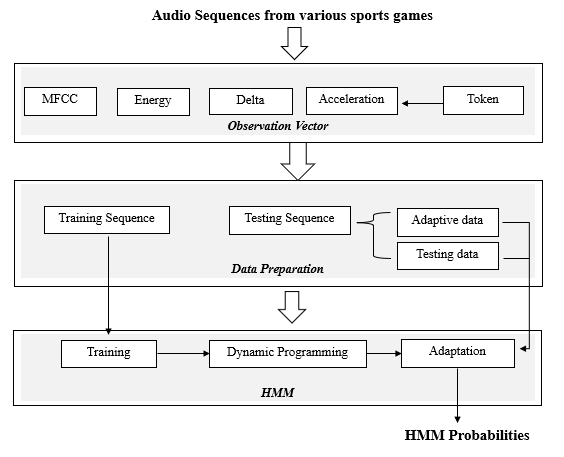
\includegraphics[width=1.0\linewidth]{Chapters/Figures/KeywordsSystemHMM.png}
        \caption{\gls{HMM}-based audio keyword generation system (adapted from \cite{AudioKeywordsSportsAnalysis})}
        \label{fig:HMM-based_keywordGenerator}
    \end{figure}

    This proposed system was then put to the test. The experimental audio data came from tennis, soccer, and basketball game videos with a total length of 2 hours. To analyze the influence of different \gls{HMM} structures and different sample sequence lengths on the performance of the systems as one was conducted some experiments, resulting in a 4-state left-right structure. For audio keywords that were of short duration, like whistling and the rebound of a ball in the courts, a length of 0.2 seconds was chosen, but for those related to speeches and interactions of the audience, it was selected a length of 1 second. The ones with a longer length are closely related to moments of high intensity and excitement, so it is used for highlight detection, thus the demonstration emphasized the generation of excited commentator speech and excited audience. In Table \ref{tab:ExperimentalResultsHMMbasedKeywords}, were listed some partial experimental results that show the efficiency of this system when compared with the previous system (frame-level \gls{SVM} keyword classification) in Basketball videos. The improvement of 5\% in the recall and precision of those keywords related to highlight detection indicates a better performance of the newly developed system.

    \begin{table}[htbp]
        \centering
        \begin{tabular}{|c|c|c|c|}
        \hline
        \rowcolor[HTML]{C0C0C0} 
        {\ul \textbf{Audio keywords}}                                       & {\ul \textbf{Methods}} & {\ul \textbf{Recall (\%)}} & {\ul \textbf{Precision (\%)}} \\ \hline
        \cellcolor[HTML]{EFEFEF}                                            &\gls{SVM}                    & 99.45                      & 99.45                         \\ \cline{2-4} 
        \multirow{-2}{*}{\cellcolor[HTML]{EFEFEF}{\ul Whistling}}           &\gls{HMM}                   & 100                        & 100                           \\ \hline
        \cellcolor[HTML]{EFEFEF}                                            &\gls{SVM}                   & 83.71                      & 79.52                         \\ \cline{2-4} 
        \multirow{-2}{*}{\cellcolor[HTML]{EFEFEF}{\ul Audience}}            &\gls{HMM}                   & 95.74                      & 95.74                         \\ \hline
        \cellcolor[HTML]{EFEFEF}                                            &\gls{SVM}                    & 79.09                      & 78.27                         \\ \cline{2-4} 
        \multirow{-2}{*}{\cellcolor[HTML]{EFEFEF}{\ul Commentator}}         &\gls{HMM}                   & 98.04                      & 94.34                         \\ \hline
        \cellcolor[HTML]{EFEFEF}                                            &\gls{SVM}                   & 80.14                      & 81.17                         \\ \cline{2-4} 
        \multirow{-2}{*}{\cellcolor[HTML]{EFEFEF}{\ul Excited Audience}}    &\gls{HMM}                    & 85.71                      & 85.71                         \\ \hline
        \cellcolor[HTML]{EFEFEF}                                            &\gls{SVM}                   & 78.44                      & 82.57                         \\ \cline{2-4} 
        \multirow{-2}{*}{\cellcolor[HTML]{EFEFEF}{\ul Excited Commentator}} &\gls{HMM}                    & 86.67                      & 100                           \\ \hline
        \end{tabular}
        \caption{Comparison between \gls{HMM} and \gls{SVM} in detecting some of the audio features
present in a basketball video (adapted from \cite{AudioKeywordsSportsAnalysis})}
        \label{tab:ExperimentalResultsHMMbasedKeywords}
    \end{table}
    
\subsection{Textual features Analysis in Sports videos}

    The \gls{OText} present in sports videos can be divided into scene and superimposed text \cite{SOCCER_VIDEO_EVENT_DETECTION}. The former refers to text that appears naturally in the recording environment, such as names on players' jerseys, slogans on banners, the result of the game, and text messages identifying that a character of a player has been slain by another \cite{SOCCER_VIDEO_EVENT_DETECTION} \cite{BroadcatedGames_analysis_LOL}. The latter is text artificially overlaid onto the video using dedicated hardware and/or software, such as the chat where the viewers and streamers interact as depicted in Figure \ref{fig:TwitchStreamStructure} or the result of tagging webcast text in Baseball videos \cite{WebcastText_Baseball_Videos} or information about the rules of the game \cite{FusionAVFeatures_ExternalInformationSources}.

    The article \cite{FusionAVFeatures_ExternalInformationSources} proposes a framework for event detection in American Football and Soccer videos that utilizes both audio and visual features analysis combined with a system to extract information from external sources. The visual feature analysis is used to detect players' trajectories, positions, and interactions, as well as the ball. Combined with the audio features analysis that captures the commentary, crowd noise and players' verbal interactions creates the \gls{AV} features analysis. The authors also proposed to incorporate external information sources to improve the event detection accuracy. These sources vary from the knowledge base of sports rules to rule out certain events as improbable or impossible, to the identification of the players that are actively on the court to rule out players that cannot be in the field and therefore cannot be tracked. To combine the \gls{AV} features with the external sources of information the system proposed refers to a \gls{FoF} and to a \gls{FoD} processes. The \gls{FoF} process refers to the process of combining the \gls{AV} features with the external sources before sending them as inputs to a classifier, such as Fisher's Linear Discriminant algorithm \cite{LinearDiscriminantAnalysis}. The \gls{FoD} process refers to combining individual classifiers, such as stacked \gls{SVM} and bagging algorithms. A third system is also proposed, the fusion of rank lists that uses a proposed algorithm of the article \cite{OptimalMultimodalFusion}.

    The work in \cite{OTRecognition_SoccerConcepts} presents a solution to \gls{OText} Recognition applied to Soccer keywords, a solution fraught with challenges such as motion blur, occlusion, and variations in font and text size. The proposed method involves pre-processing video frames to mitigate noise and enhance contrast. Subsequently, a text detection algorithm is employed to pinpoint and extract the overlaid text. This process involves the application of the Sobel operator to the original frame. The complete process is described in Figure \ref{fig:OT_ExtractionRecognition}.

    \begin{figure}[htbp]
        \centering
        \fboxsep=0pt\fboxrule=0.5pt
        \fbox{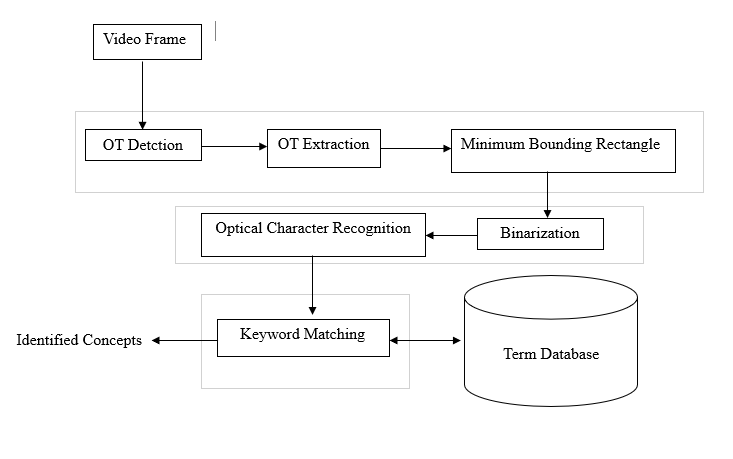
\includegraphics[width=0.8\linewidth]{Chapters/Figures/OT_ExtractionRecognition.png}}%
        \caption{Complete process of \gls{OText} extraction and recognition (adapted from \cite{OTRecognition_SoccerConcepts})}
        \label{fig:OT_ExtractionRecognition}
    \end{figure}

    The Sobel operator \cite{SobelOperator} is a renowned technique for edge detection. It effectively identifies the sharp transitions in brightness that delineate the boundaries between objects and regions within an image. It utilizes two 3x3 masks, one for horizontal and one for vertical edges. Each mask contains positive and negative values arranged in a specific pattern that emphasizes the intensity gradient along a particular direction.

    Subsequently, the obtained image undergoes element dilation, binarization, and morphological opening processes \cite{MorphologicalTransformations}. Finally, the textual information is encapsulated by boxes through component analysis.

    With the regions of \gls{OText} already identified, it is now necessary to apply a technique to recognize the text. The technique used in the article is the \gls{OCR} technology \cite{OverviewTesseractOCREngine}. This technology is responsible for converting the image of a text into machine-encoded text, and its performance is increased accordingly with an increase in the contrast between the background and the letters, thus the use of the process of binarization \cite{ThresholdSelectionMethod}.

    The devised approach to extract and identify overlaid text in soccer videos yields a collection of textual attributes suitable for event detection. These features, acquired using \gls{OCR} technology, can be cross-referenced with a predefined set of soccer-related keywords. Furthermore, the \gls{OCR} system can identify numerical values within the score marker, offering a valuable verification mechanism for event detection. This facilitates a precise determination of when significant events, such as goals or points, take place during the match.

\section{Event detection and Highlight detection in Video games}

    In this section, we will present two solutions for event detection and highlight detection in Video games. One uses an automatic feature analysis approach \cite{BroadcatedGames_analysis_LOL} and the other uses a tool adopted by industry-leading graphics engines such as  Unreal Engine 4.18 and Unity 5.6 to capture and share a gamer's bet moments \cite{NVIDIA_GeForce}.  

\subsection*{Game engine integrated tools - NVIDIA Highlights}
    
    NVIDIA Highlights is a feature of GeForce Experience \cite{NVIDIA_GeForce} that automatically captures and saves in-game highlights for compatible games, and this cutting-edge highlight recording tool has been crafted through collaboration between NVIDIA and top-tier graphics engines in the industry. This tool empowers game developers to indicate key highlights during gameplay, triggering the creation of a video sequence from the player's viewpoint. Integrated seamlessly into Unity and Unreal, NVIDIA Highlights can also be implemented in other engines using their respective SDKs.

\subsection*{Automatic feature analysis approach}

    This article \cite{BroadcatedGames_analysis_LOL} proposes a framework for event detection and highlight detection in \gls{LOL}. 
    
    In video games like \gls{LOL} important events can be identified through all the types of \gls{LLF}. To infer the game progress of each session the system developed uses a similar approach as \cite{OTRecognition_SoccerConcepts}. For each video frame, is applied a preprocessing to detect \gls{ROI}, the Sobel edge detector to detect all the edges, and binarization to filter out the weak ones. Next, the morphological operations such as dilation and erosion filter out more weak edges and minimize the number of bounding boxes by eliminating the ones that are smaller than the minimum. Finally, it is employed the Tesseract OCR package to recognize text in each detected bounding box. When comparing the text resulting from the \gls{OCR} with the set of predefined sentences from the table with the domain knowledge it results in a non-match that box will be discarded. But when it matches the text will be used to represent an event.

    The same article also depicts a system to detect highlights in a video game feed. This system extracts features from both the video and viewers and uses them to construct models based on a psychological approach and a data-driven approach, respectively. From the video segment, it is possible to extract features like motion intensity that increases accordingly with the peak interest that visual content can bring, frame dynamics that indicate possible visual effects like when invoking an ability, number of player characters that might indicate a group fight between the players, event ratio that indicates that if multiple import events are occurring in such short time it means that must be a highlight in creation, number of viewers chat that indicate that if a burst of chats messages occur it means that it is occurring a highlight, and the same applies to emojis in the chat. 

    

